
\chapter{Deep learning}
In this chapter we are going to introduce deep learning, methods of which are going to be implemented in our solution. We will introduce general principles and take a closer look on artificial neural networks, with main focus on convolutional neural networks. Lastly, the topic of interpretability and explainability of neural networks is discussed, with an emphasis on Layer-wise Relevance Propagation.

Deep learning is a form of machine learning, which is a significant part of the scientific field known as artificial intelligence. Over the past decade, a remarkable progress has been made in application of machine learning systems in numerous fields of science as well as in everyday life \cite{longsurvey2018}. They are used in natural language processing, detection of objects in images or speech recognition. These systems thrive mainly because of growing amounts of available data and empowerment of fast GPU computing, both of which is important for their proper training. The usage of machine learning in medicine benefits primarily from ascending volume of digitalized patient data. In 2017 in the United States alone, 150 exabytes of medical data was generated and this number increases annually by approximately 47\% \cite{stanford2017}. With that said, deep learning systems are able to move from theory to practice and assist physicians in hospitals and health centers. According to Stanford Medicine Health Trends Report of 2020 \cite{stanford2020} up to June 2019, the U.S. Food and Drug Administration had approved a total of 46 machine learning algorithms for medical purposes. As machine learning and its applications is still being explored, we can expect this number to further increase rapidly.

Deep learning enables computational models, which are composed of several processing layers, to learn representations of data, which contain multiple  underlying levels of abstraction \cite{greekDeepLearning}. It allows computers to learn from experience and comprehend the world more like a human - as a hierarchy, where complicated concepts are composed of more simple ones. \cite{deeplearningbook} The conventional machine learning approach required a human expert to do a hand-crafted engineering to extract features from data prior to feeding it to a machine, which required much more time and resources. The key advantage of deep learning is that the features are learned by the machine automatically, thanks to a data-driven approach throughout the learning process \cite{deeplearningHealthcare}. 



\section{Deep learning categorization}
We distinguish several primary forms of machine learning, which can be applied to deep learning as well. The main two, which we will discuss in our work, are supervised and unsupervised learning.  \cite{lecundeeplearning} These two forms differ mainly in whether labeled data, corresponding to the input data, is available for the training process. There is a form of learning known as semi-supervised, which we will, however, not further discuss.

\subsection{Supervised learning}
Supervised learning  is the most frequently used form of machine learning \cite{lecundeeplearning}. As it's name suggests, systems which fall under this category are trained under a certain form of supervision, which is present to guide the learning process. During training, a function is computed after each prediction, which measures the error rate of the model. According to the computed value, the internal parameters of the machine are adjusted in order to minimise the error rate in future predictions. These adjustable parameters are the model's most important component. A procedure which empowers nearly all deep learning models' error rate computation and ensures the parameter adjustment is called Stochastic gradient descent. We will discuss this procedure in more detail later in this chapter. Classification and regression are the two main tasks, which supervised learning attempts to solve \cite{kim2019deep}. Our solution will work with labeled data, thus it falls under the category of supervised learning.

\subsection{Unsupervised learning} The technique used by unsupervised learning algorithms is to learn important features contained in the training data without any supervision, as the name implies \cite{deeplearningbook}. Unsupervised learning model attempts to automatically discover the underlying information by extracting and analyzing useful features. This type of learning does not require the training data to be labeled with the correct answer. In this matter embodies it's biggest advantage - withdrawal from the need of labeled data, which would require manual intervention and is not always easy to obtain. Although there is no distinct line between supervised and unsupervised concepts, we can say that the most widely used unsupervised learning algorithms are clustering, principal components analysis, anomaly detection or generative adversarial networks \cite{deeplearningbook, kim2019deep}.

\section{Artificial neural networks}
This section is primarily dedicated to deep neural networks, which are the core of our solution. However, in order to gain better perspective, we will first introduce some conceptual and historical context of artificial neural networks in general.\\
Proposed in the 1940s, artificial neural network (ANN) is a computational model, which is a part of the broad artificial intelligence field. The word "neural" refers to the fact, that it was initially inspired by the way human brain functions. There are approximately $10^{11}$ neurons inside a human brain \cite{navrat2007umela}. Neuron is an elementary cell of the neural system, in which biochemical processes ensure the possibility of processing and sending neural signals. These signals are often referred to as activations. Neurons are interconnected by special joints called synopses, which enables them to communicate \cite{navrat2007umela}. Throughout the whole life, the importance and strength of synopses between neurons change, impacted by human's experience and learning. Artificial neural networks simulate the structure, as well as the behaviour of neurons. If we were to apply the biological terms to an ANN, synopses would be called weights
\subsection*{Perceptron} 
Perceptron is the earliest model of a neural network, composed of a single neuron. The output \textit{o} of the perceptron is defined by the following formula:
\begin{equation}
    o = f(net) = f(\bar w \cdot \bar x) = f (\sum_{j=1}^{n+1} w_jx_j)
\end{equation}
where $f$ is the activation function, $\bar w$ is the weights vector, $\bar x$ is a vector of the input signals. This perceptron calculates with having $n+1$ inputs \cite{navrat2007umela}. The abilities of a single perceptron are quite constrained. It only manages to classify input data into two separate classes. With that said, perceptron provides a solution only to linearly separable problems \cite{navrat2007umela}.
\subsection*{Feedforward neural networks}
Most real-world problems do not have linear character and can not be tackled with the simple perceptron model. A solution to this problem was introduced in 1980s when feedforward neural networks with the backpropagation algorithm were proposed \cite{navrat2007umela}. Multiple neurons (perceptrons) arranged in layers is what constructs a feedforward neural network. In this type of network, the information is passed only in the forward direction and the connections between neurons form a directed acyclic graph. In other words, each neuron from layer \textit{l} sends signals to each neuron in layer \textit{l+1}. The very first (leftmost) layer in a network is called input layer and the last (rightmost) is called output layer. In between, one middle layer, often also called "hidden" layer, is situated. 
\begin{figure}[!ht]
\centering
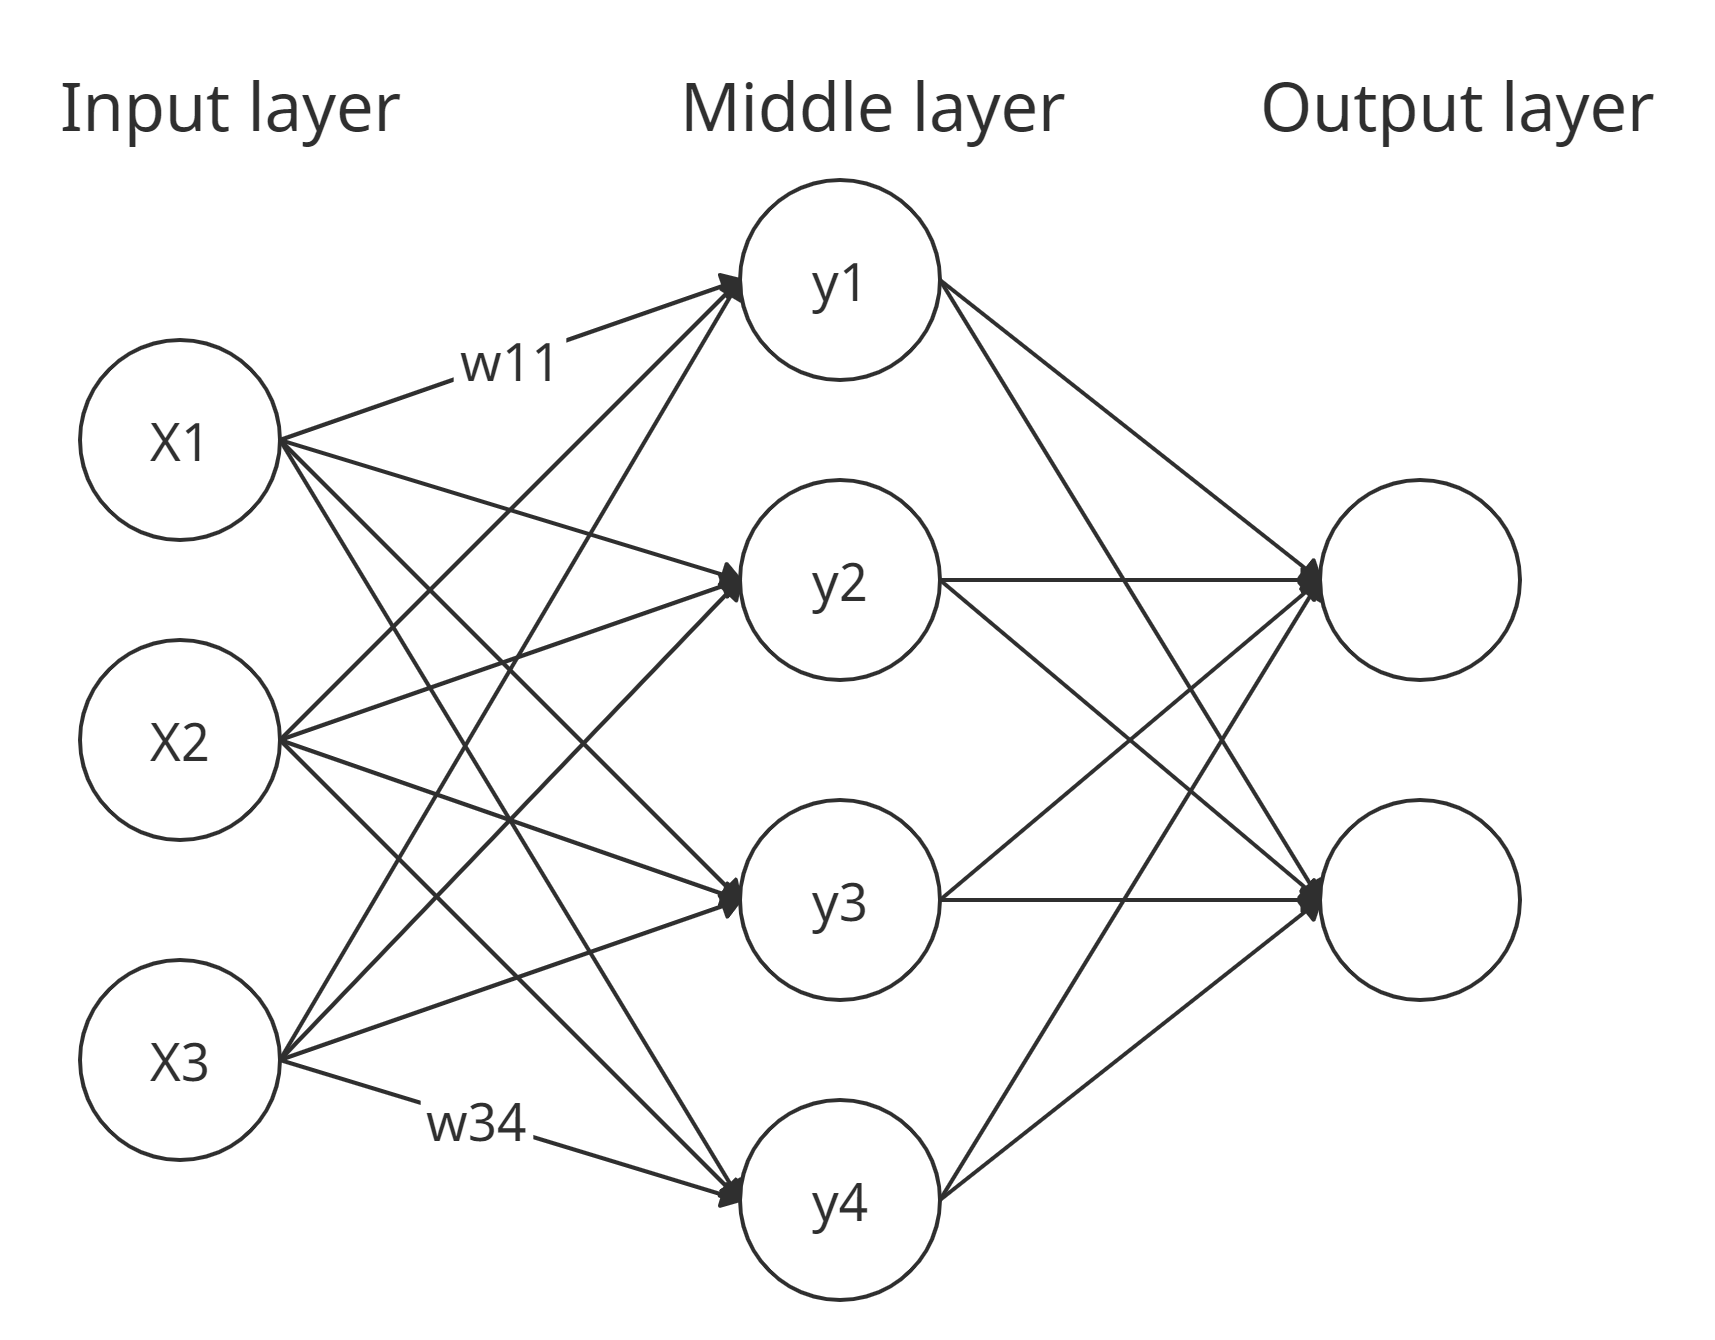
\includegraphics[width=7cm]{assets/images/FFN}
\caption{Architecture of a feedforward neural network
\label{fig:FFN}}
\end{figure}
\\At each layer a calculation is performed, which involves computing a weighted sum of the neuron's input values, followed by a functional operation. Performing this operation equals to applying a nonlinear activation function to the previously computed weighted sum \cite{tutorialIEEE}. The following formula is used at each layer:
\begin{equation}
    y_{j}=f\left({\sum \limits _{i=1}^{n} w_{ij} \times x_{i} + b}\right)
\end{equation}
where $y_j$ is the input value for j-th neuron in corresponding - in this case the middle - layer, $w$ are the weights, $x$ is the value of a neuron from previous layer, $b$ is the bias term and $f$ is the activation function, same as with perceptron mentioned earlier \cite{tutorialIEEE}. The main purpose of bias is to assign each neuron in a network a constant, which would be adjustable by training. The variable $n$ refers to the number of neurons in the previous (input) layer.
\subsection{Deep neural networks}
In the neural networks domain, deep neural networks (DNN) introduce the use of deep learning in a neural network model. This type of neural network differs from the one introduced in previous section in having more than one hidden layer. 
\begin{figure}[!ht]
\centering
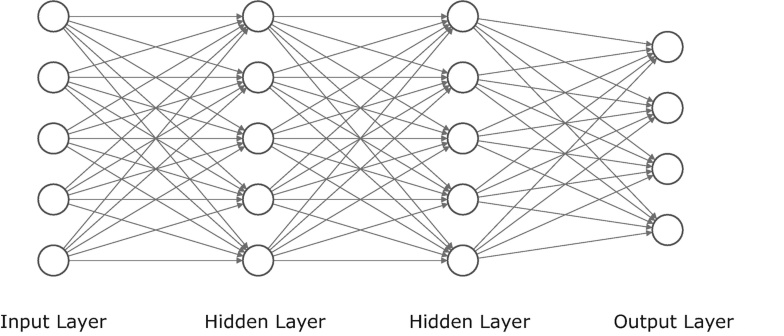
\includegraphics[width=12cm]{assets/images/DNN1}
\caption{Architecture of a deep neural network with two hidden layers \footfullcite{chapterBookDL}
\label{fig:DNN}}
\end{figure}

\subsubsection{Activation functions}
For deep neural networks to learn to solve real problem, it is important to introduce nonlinearity into the computational process during training \cite{tutorialIEEE}. This requirement is fulfilled by activation function. There are three historically most frequently used activation functions, each of which is advantageous for a different task.
\begin{figure}[!ht]
\centering
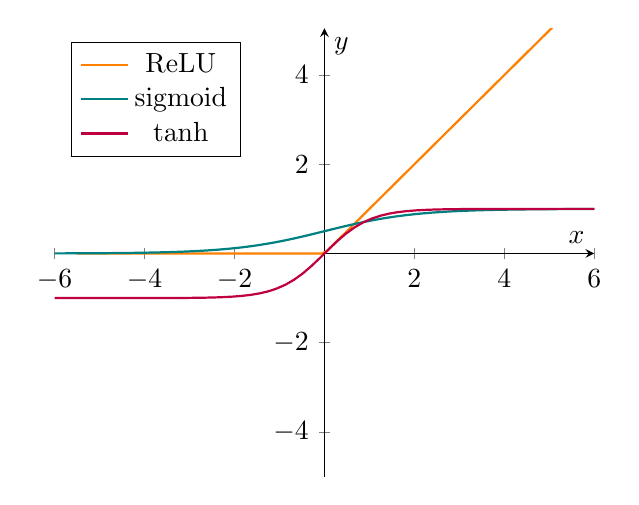
\begin{tikzpicture}
\begin{axis}[
    axis lines=middle,
    xmax=6,
    xmin=-6,
    ymin=-5,
    ymax=5.05,
    xlabel={$x$},
    ylabel={$y$},
    legend pos=north west]
\addplot [domain=-5.5:5.5, samples=100, thick, orange] {max(0, x)};
\addplot [domain=-9.5:9.5, samples=100,
          thick, teal] {1/(1+exp(-x)};
\addplot [domain=-9.5:9.5, samples=100,
     thick, purple] {(exp(x) - exp(-x))/(exp(x) + exp(-x))};
\legend{ReLU, sigmoid, tanh}
\end{axis}
\end{tikzpicture}
\caption{Activation functions graph
\label{fig:activationFunctions}}
\end{figure}
\subsubsection*{Rectified linear function}
Rectified linear or ReLU is the activation function of choice in modern neural networks \cite{tutorialIEEE}. It is defined as:
\begin{equation}
     f(x) = max\{0, x\}
\end{equation}
where we can see, that this function outputs zero if $x\leq0$, otherwise the output is $x$ \cite{deeplearningbook}. However, the fact that it automatically maps all negative values to zero results in decreasing the ability of the DNN to learn properly. Due to this issue, several variations of ReLU were proposed, such as leaky ReLU or parametric ReLU \cite{tutorialIEEE}.

\subsubsection*{Sigmoid function}
The sigmoid function takes an input $x$ and suppresses it to a value from range $[0,1]$, as can be seen in its notation:
\begin{equation}
    f(x) = \sigma(x)=\frac{1}{1+e^{-x}}
\end{equation}
Taking into account its output range, sigmoid is especially beneficial to models, which predict a probability.

\subsubsection*{Hyperbolic tangent function}
The hyperbolic tangent function is similar to sigmoid, however its ouput range is wider. 
\begin{equation}
    f(x) = \tanh(x)=\frac{e^x-e^{-x}}{e^x+e^{-x}}
\end{equation}
This function maps the input $x$ into a value from range $[-1,1]$.
\subsubsection{Backpropagation algorithm}
An optimization technique is what powers the deep learning process. When training a network, we want to minimize average loss, which is the difference between desired output and the current output of the network. It is highly dependable on the weights' adjustment. Updating the weights is executed by computing the gradient descent, through the process of backpropagation \cite{tutorialIEEE}.

\subsubsection*{Stochastic gradient descent}
Stochastic gradient descent is probably the most popular algorithm used for optimization. It is based on the simpler Gradient descent algorithm, which uses the computation of the first derivative to find a global minimum of a function \cite{deeplearningbook}. Let $w_ij^t$ be a weight value at a specific time point, $L$ is the loss and $\alpha$ the current learning rate, we can then compute the update value of the weight as follows:
\begin{equation}
w_{ij}^{t+1} = w_{ij}^{t} - \alpha \frac {\partial L}{\partial w_{ij}}   
\end{equation}
Computing the derivative gives the answer to the question of how the model should adjust its parameters in order to improve its predictions. The word "stochastic" refers to the fact, that instead of all data samples, for each iteration only a few samples are randomly selected for the computation.



\subsection{Convolutional neural networks}
Convolutional neural network (CNN) is a special kind of feedforward neural network, where the convolution operation is used instead of classical matrix multiplication \cite{deeplearningbook}. It was introduced as a method of efficiently handling grid-like data such as images and videos, as it is able to successfully capture the spatial and contextual dependencies within these kinds of 
multi-dimensional data. CNNs have been initially inspired by the functioning of primary visual cortex, located in the bottom back area of the brain \cite{deeplearningbook}.
\subsubsection{Layer architecture}
Convolutional neural network comprises three main different kinds of layers, each of which performs a different role: convolutional layer, pooling layer and fully connected layer.
\begin{figure}[!ht]
\centering
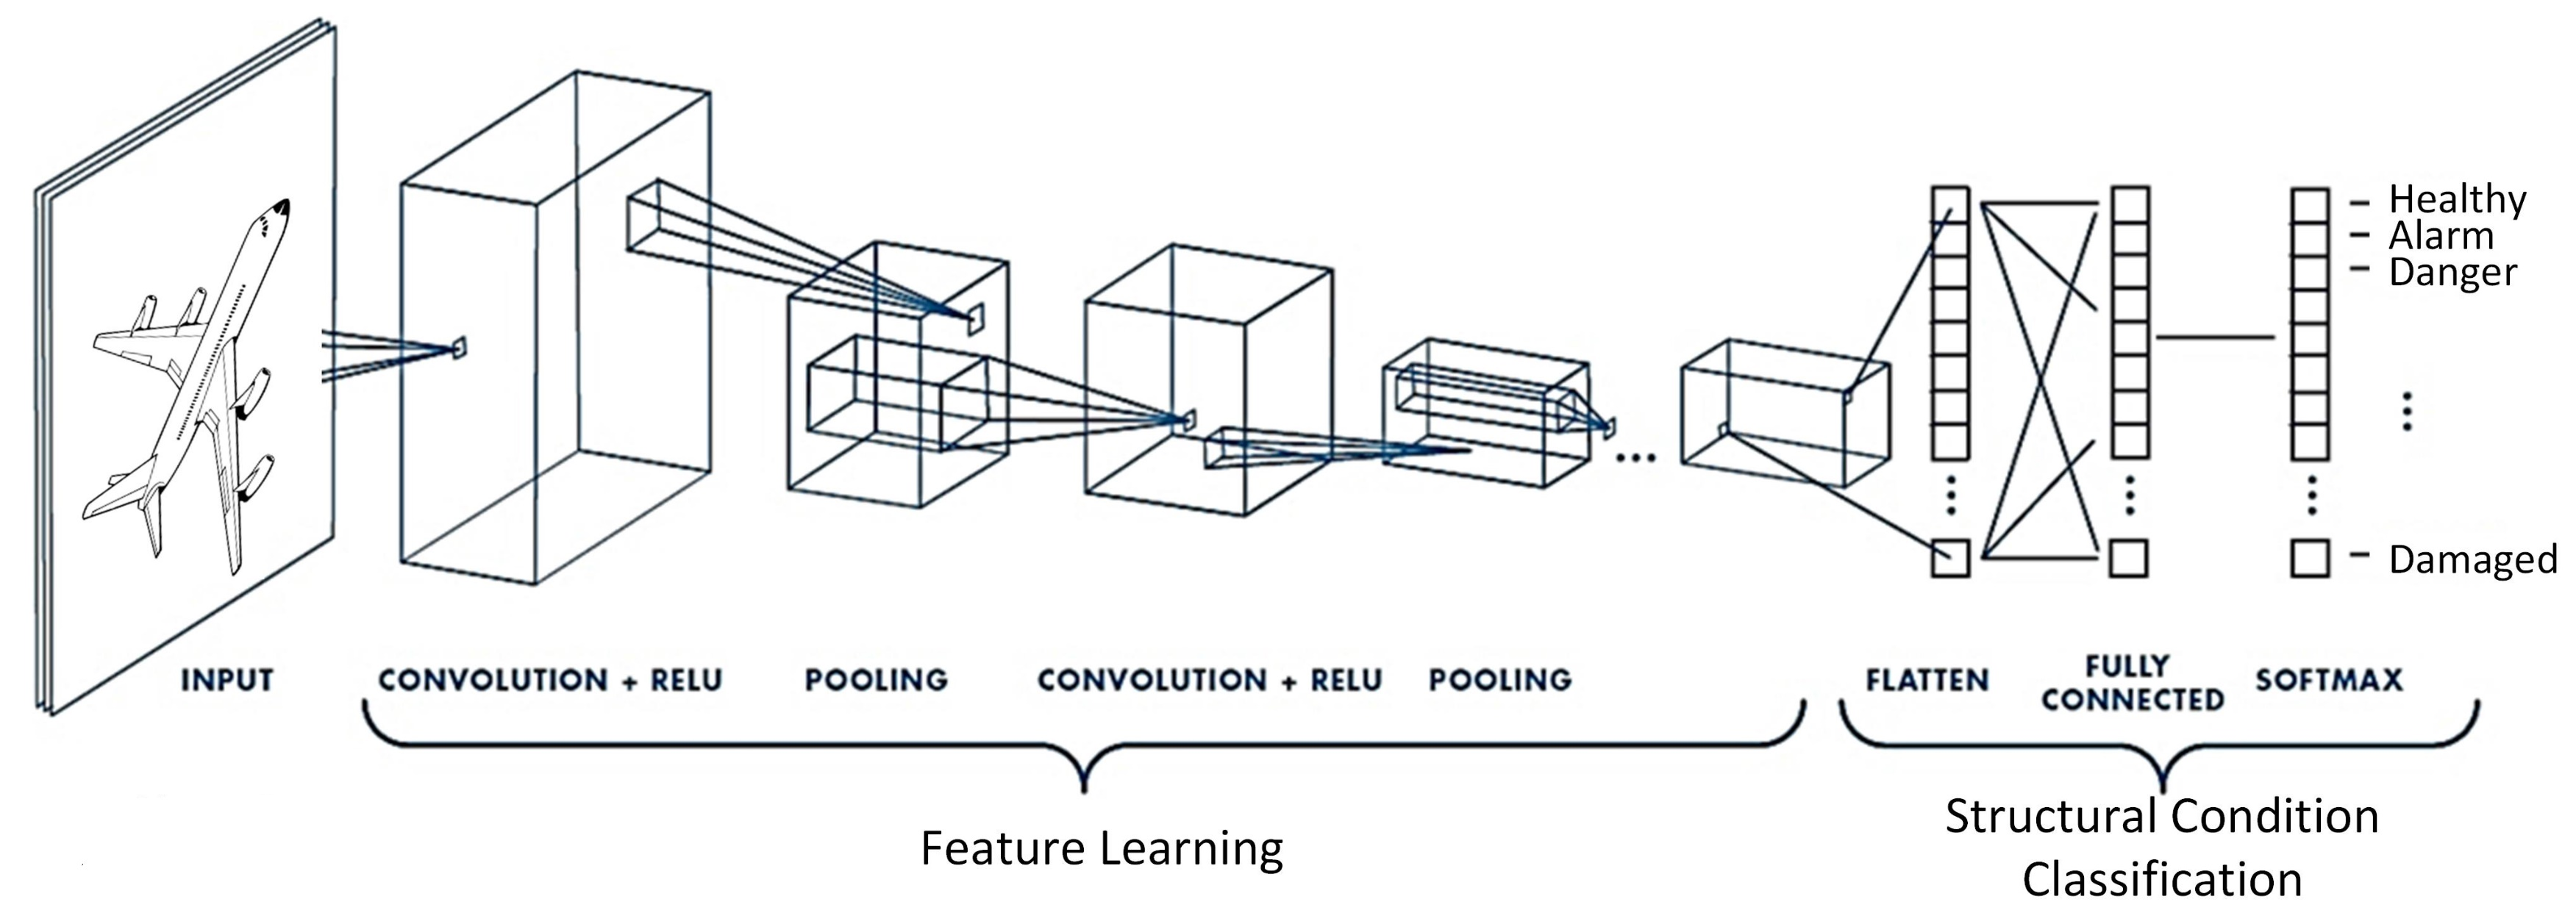
\includegraphics[width=15cm]{assets/images/CNN}
\caption{Example of a convolutional neural network architecture \footfullcite{CNNpicture}
\label{fig:CNN}}
\end{figure}

\subsubsection*{Convolutional layer}
Convolutional layers are the most important building blocks of a CNN, since they perform the convolution operation, as their name implies. The element accountable for the convolution operation is called a kernel or filter, gradually which slides over the input image. To carry out a convolution basically means to compute matrix multiplication between kernel and the part of the input image, which is currently overlapped by the kernel. As a result of this operation, an output feature map is generated \cite{greekDeepLearning}. The objective of this layer is to detect associations between features passed from the previous layer \cite{lecundeeplearning}. After each convolution layer an activation function, such as ReLU, is applied to introduce nonlinearity.

\subsubsection*{Pooling layer}
A convolutional layer is typically followed by pooling layer. We use pooling to reduce the spatial dimensions through down-sampling of the feature maps. It also enables the network to be invariant to small translations \cite{deeplearningbook}. Different strategies of pooling can be used, namely max pooling or average pooling, returning either the maximum value or the average value from the part of the feature map covered by the kernel respectively \cite{lecundeeplearning}.
\subsubsection*{Fully connected layer}
After several stagies of convolutional a pooling layers, fully connected layer is the one which performs the high-level feature reasoning. In other words, this layer combines features detected in previous layers and thus learns the nonlinear representations in data \cite{greekDeepLearning}. In order to present a 1D vector as the final output, the 2D feature maps are flattened. This flattened vector is then either classified using the softmax classification technique or used for further processing.
\subsubsection{Main concepts}
CNNs greatly benefit from three main concepts: sparse connectivity, equivariant representations and shared parameters. We will discuss each of these separately.
\subsubsection*{Sparse connectivity}
The main motive of sparse connectivity (also sometimes referred to as sparse weights) is the absence of the traditional scheme of connecting each neuron from one layer to each neuron in the previous layer, as it was introduced in traditional feedforward networks \cite{chapterBookDL}. A neuron in convolutional network only interacts with a few other neurons, which can significantly reduce memory requirements as well as improve computational efficiency \cite{deeplearningbook}. In CNN this concept is secured by using a kernel (filter) of a smaller size compared to the size of the input data. Even though the connections in CNN are sparse, neurons in deeper layers are able to interact with input values indirectly. Moreover, deeper situated neurons have larger receptive field compared to neurons in shallow layers, which empowers the network to "efficiently describe complicated interactions between many variables by constructing such interactions from simple building blocks that each describe only sparse interactions" \cite{deeplearningbook}.
\subsubsection*{Shared parameters}
Sparse connectivity closely relates with another concept called shared parameters. It refers to reusing the same set of weight values when calculating the output for a set of neurons \cite{greekDeepLearning}. From the learning point of view, using shared parameters equals to learning only one set of parameters, instead of a separate one for every location of the input \cite{deeplearningbook}. The neurons in a layer that share the same set of weights form a plane. Each plane is then responsible for learning a specific feature \cite{greekDeepLearning}. This concept can reduce memory consumption as well.
\subsubsection*{Equivariant representations}
The last concept, which we will introduce, is equivariant representations, or equivariance in translation. It ensures, that if an input image is changed by any action, the output, generated by convolution operation, changes equivalently to the distortion \cite{deeplearningbook}. This is caused by previously mentioned concept of parameter sharing. Common mathematical definition for equivariance to translation is $f(g(I)) = g(f(I))$, where $I$ represents the input image, $g$ stands for the function executing a distortion and $f$ is the convolution operation.

\section{Interpretability and explainability of neural networks}
As machine learning models constantly work forward and excel in many tasks, a question regarding their trust and transparency arose. They are commonly being addressed as "black boxes", due to the fact, that their arrival at predictions is highly non-transparent \cite{explainDLbook}. In some areas of AI applications, namely those which are part of basic everyday life, such as entertainment or e-commerce, the potential failure of these ML models is rather insignificant, without any serious consequences. However, this can not be applied to domains such as medicine and healthcare, where the life of patients' is at stake. The field of explainable artificial intelligence is dedicated to addressing this challenge \cite{explainDLbook}. For implementing AI models into clinical routine, where they usually maintain a supportive role in the diagnostics process, it is crucial to provide physicians explanation of the model's prediction, to gain more trust and reliability. We will now take a closer look on one of the methods recently explored in explainability of deep learning models.
\subsection{Layer-Wise Relevance Propagation}
Layer-wise Relevance Propagation (LRP) is an algorithm, used in general neural network structures to introduce explainability. In \cite{explainDLbook} it is stated, that "LRP explains individual decisions of a model by propagating the prediction from the output to the input using local redistribution rules". It simply means, that after the neural network makes a prediction, a backward pass through its neurons is conducted, and neurons, which contributed the most to the prediction, are identified \cite{explainDLbook}. As a result a heatmap with most important pixels highlighted is generated.
If $j$ and $k$ are neurons at two neighbouring layers of a neural network, $z_jk$ poses the extent to which neuron j has contributed to make neuron k relevant, then $(R_k)_k$, which is the relevance score at a given layer propagated onto neurons from the lower layer, can be achieved by applying following formula \cite{explainDLbook}:
\begin{equation}
 R_j = \sum _k \frac{z_{jk}}{\sum _{j} z_{jk}} R_k   
\end{equation}

\begin{figure}[!ht]
\centering
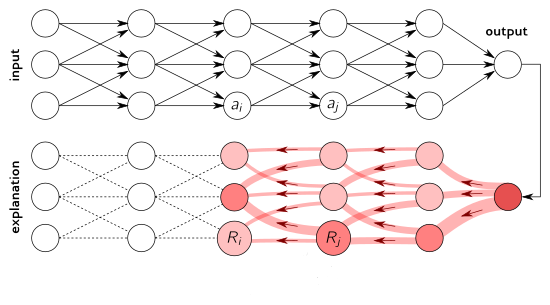
\includegraphics[width=10cm]{assets/images/LRP}
\caption{The LRP procedure \protect\footnotemark}
\end{figure}
\footnotetext{www.heatmapping.org}



